
\documentclass[a4paper,12pt]{article}
\usepackage[top=1in,bottom=1in,left=1in,right=1in]{geometry}
\usepackage[T1]{fontenc}
\usepackage[utf8]{inputenc}
\usepackage{newunicodechar}
\usepackage{lmodern}
\usepackage{textgreek}
\usepackage{amsmath}
\usepackage{mathtools}
\usepackage{graphicx}
\usepackage{pdflscape}
\usepackage{svg}


\usepackage{tabularx}
\usepackage{blindtext}
\usepackage{hyperref}
\usepackage{pgfgantt}
\usepackage{colortbl}
\usepackage{pdfpages}
\usepackage{setspace}
\usepackage{subcaption}
\usepackage{tikz}
\usepackage{chngcntr}
\usepackage{longtable}
\usepackage{xcolor,colortbl}
\usepackage{pdfpages}
\counterwithin{figure}{subsection}
\usepackage{multicol} 

\setcounter{tocdepth}{3}


\usepackage[backend=bibtex]{biblatex}
\addbibresource{references.bib}


\begin{document}

	\begin{titlepage}
		\newcommand{\HRule}{\rule{\linewidth}{0.5mm}}
		\begin{tikzpicture}[remember picture, overlay]
		\node [anchor=north east, inner sep=0pt]  at (current page.north east)
		{
\includegraphics[width=21cm]{graphics/ucl-banner-dl-port-outline.eps}};
		\end{tikzpicture}\\[3cm]
		\center
		
		\textsc{\Large University College London}\\[0.5cm]
		\textsc{\large Department of Electronic and Electrical Engineering}\\[0.5cm]
		
		\HRule \\[0.4cm]
		\setstretch{1.5}
		{ \huge \bfseries Performance characterisation of 8-bit RISC and OISC architectures}\\[0.4cm]
		\setstretch{1.0}
		\HRule \\[1.0cm]
		
		\begin{multicols}{3}
			
		\Large \emph{Author:}\\
		Mindaugas \textsc{Jarmolovicius}\\
		\href{mailto:zceemja@ucl.ac.uk}{zceemja@ucl.ac.uk}\\
		
		\columnbreak
		
		\Large \emph{Supervisor:}\\
		Prof. Robert \textsc{Killey}\\
		\href{mailto:r.killey@ucl.ac.uk}{r.killey@ucl.ac.uk}
		
		\columnbreak
		
		\Large \emph{Second Assessor:}\\
		Dr. Ed \\\textsc{Romans}\\
		\href{mailto:e.romans@ucl.ac.uk}{e.romans@ucl.ac.uk}
		
		\end{multicols}
		
		\vfill
		\setstretch{2.5}
		{ \large \bfseries A BEng Project Interim Report}\\[1cm]
		\setstretch{1.0}
		{\large December 13, 2019}\\[2cm]
		
	\end{titlepage}

\pagebreak

\begin{multicols}{2}

\section{Abstract}
This project investigates area / performance / power / complexity benefits and trade-offs of One Instruction Set Computer (OISC) comparing to traditional Reduced Instruction Set Computer (RISC) architectures in general computing application. It is shown that \texttt{SUBLEQ} OISC performs better in special cases, however there is lack of research in more complicated OISC architectures designed for general computing. At this point project is mainly following schedule with mainly benchmark being behind the schedule.

\section{Introduction}
Since 80s there been a raise of many processor architectures that try to fulfil specific performance and power application constraints. One of noticeable cases is ARM RISC  architecture being used in mobile devices instead of more popular and robust x86 CISC (Complex Instruction Set Computer) architecture in favour of simplicity, cost and lower power consumption \autocite{jamil_1995,blem_menon_sankaralingam_2013}. Its been shown that in low power applications such as IoTs (Internet of Things), OISC\footnote{Also known as URISC (Ultimate Reduced Instruction Set Computer)} (One Instruction Set Computer) implementation can be superior in power and data throughput comparing to traditional RISC architectures \autocite{yokota_saso_hara-azumi_2017, ahmed_sakamoto_anderson_hara-azumi_2015}. This project proposes to compare two novel RISC and OISC architectures and compare their performance, design complexity and efficiency.

Project is split into 3 main objectives:\\
$\bullet$ Design and build a RISC based processor. As it is aimed for low power and performance applications this will be 8bit data size processor with 4 general purpose registers.\\
$\bullet$ Design and build an OISC based processor. There are multiple different implementations such as \texttt{SUBLEQ} or one proposed in chapter \ref{sec:theory}.\\
$\bullet$ Design a fair benchmark that both processors could execute. Benchmark may include different algorithms that are commonly used in controllers, IoT devices or similar low power microprocessor applications.

Following chapters will describe the estimated project outcome, project schedule and work done so far.

\section{The Work Performed to Date}
\subsection{Supporting Theory} \label{sec:theory}
This section explains the theory and predictions of RISC and OISC architectures.

Figure \ref{fig:simple_blocks} represents simplified diagrams of RISC and OISC architectures. In RISC and CISC architecture, program data travels from program memory to control block where instruction is decoded and further decided where what data is directed in datapath block which is described in section \ref{sec:datapath}. Such structure requires complicated control block and additional data routing blocks. In order to increase performance of such processor one would need to add pipelining or add multiple cores. Both methods bring big disadvantages - multicore processor requires software adjustments and each core doubles the control and datapath substantially increasing die area; pipelinig allow operation at higher frequencies however it brings design complications such as complicated hazard prevention logic and instruction lookup. RISC architecture is mainly based on theory in \autocite{harris_harris_2013}. Simplicity of OISC architecture overcomes these disadvantages:
\\
Pipelining can be done by individual blocks and programmibly waiting for results, this is represented in figure \ref{fig:oisc_simple} Adder and Multiply vertical blocks, multicore can be simulated by adding more data and instruction buses, hazards can be prevented with software or/and integrated into address registers.
\\ 
ALU and any other processor component can be divided by adding different address registers thus allowing to utilise multiple components at the same time given that multiple data buses are used. This is represented in figure \ref{fig:oisc_simple} Arithmetic Unit horizontal blocks. Assuming 4 data and instructions buses are used, \textbf{AND} and \textbf{OR} blocks sources A and B can be all written during one cycle utilising both blocks at the same time.
\\
These principal functions should allow OISC architecture to have advantage in performance and power consumption while having lower transistor count and this is the main motivation behind project. This expectation is supported mainly by following papers:
\\
$\bullet$ Using OISC \texttt{SUBLEQ} as a coprocessor for MIPS-ISA processor to emulate the functionality of different classes shows desirable area/performance/power trade-offs \autocite{ahmed_sakamoto_anderson_hara-azumi_2015}.
\\
$\bullet$ Comparing OISC \texttt{SUBLEQ} multicore to RISC achieves better performance and lower energy for streaming data processing \autocite{yokota_saso_hara-azumi_2017}.
\\
There is a lack of research investigating and comparing more general purpose OISC non-\texttt{SUBLEQ} processor. The main theory for OISC used in this project will be based on \autocite{ong_ang_seng_2010,gilreath_laplante_2003,kong_ang_seng_adejo_2010,dharshana_balasubramanian_arun_2016}.
\columnbreak

\end{multicols}

\begin{figure}[t!]
	\centering
	\begin{subfigure}[b]{1\textwidth}
		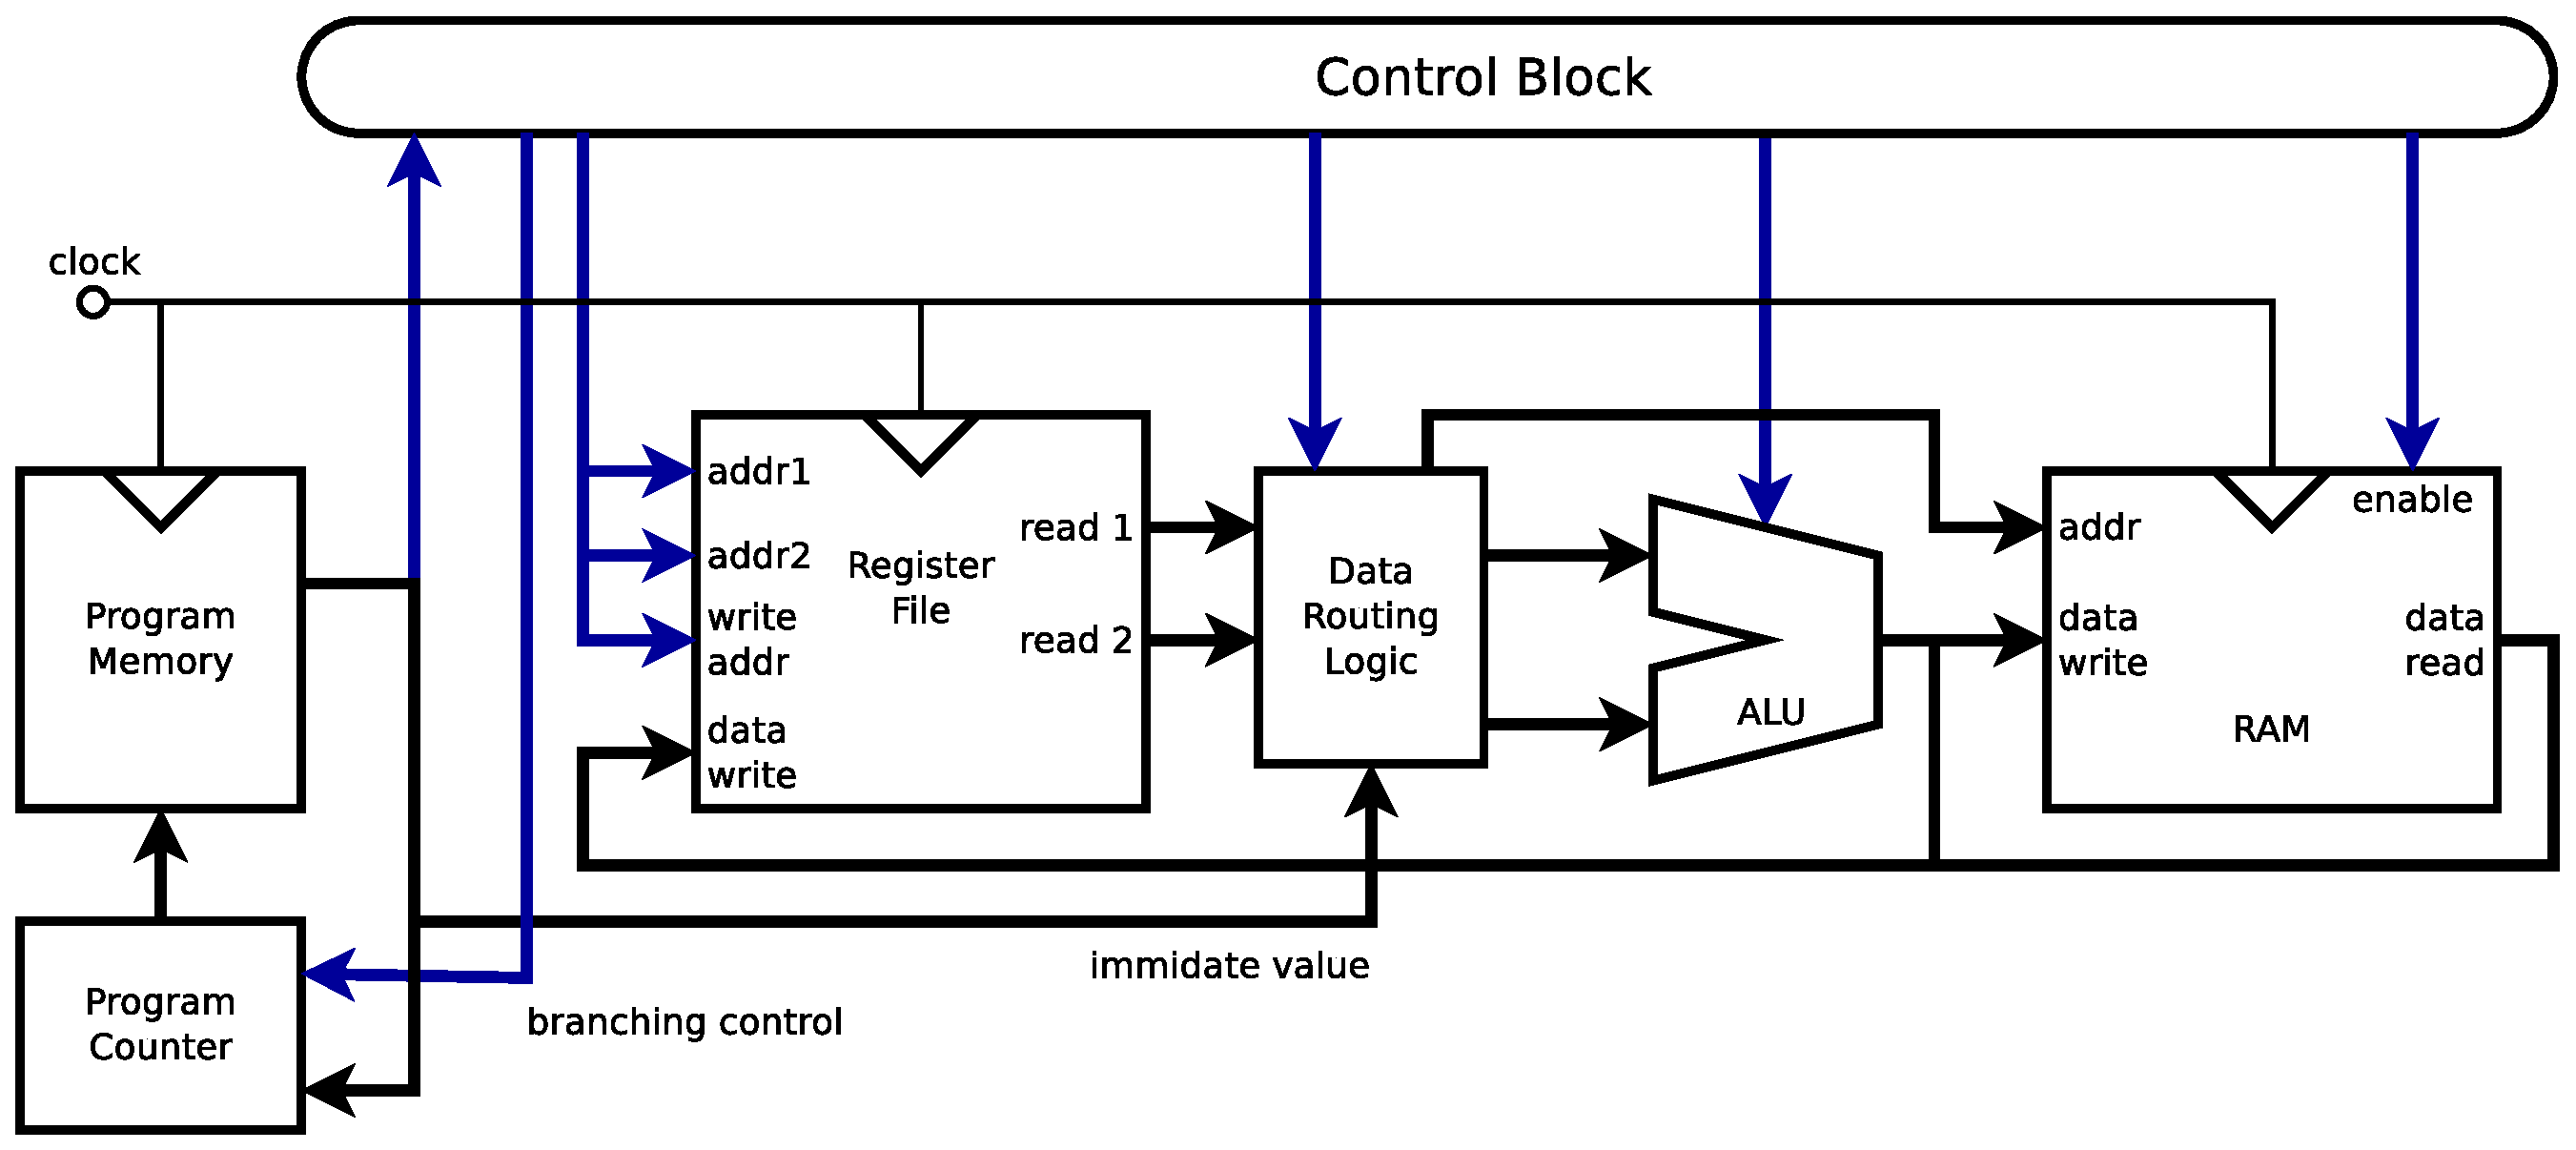
\includegraphics[width=\linewidth]{graphics/risc.eps}
		\caption{RISC microarchitecture diagram}
		\label{fig:risc_simple}
	\end{subfigure}
	
	\begin{subfigure}[b]{1\textwidth}
		\includegraphics[width=\linewidth]{graphics/oisc.eps}
		\caption{Single data bus OISC microarchitecture diagram}
		\label{fig:oisc_simple}
	\end{subfigure}
	
	\caption{Simplified diagrams of both architectures. Blue lines indicate control/instruction buses and black - data buses}
	\label{fig:simple_blocks}
\end{figure}
\newpage
\begin{landscape}
	\subsection{Project Scheduling}
	As it can be seen in table \ref{table:time} below, project is mainly split into Term 1 which is dedicated for RISC and Term 2 which is dedicated for OISC implementation. Approximately 3 weeks are left until final report to have enough spare time to finish all tests and complete poster \& report itself. It is also expected to have a lot of coursework around this time. Currently mainly benchmark development is behind schedule, more information in section \ref{sec:benchmark_issues}.
	
	\begin{table}[h!]
		\centering
		\begin{ganttchart}[
			y unit title=0.4cm,
			y unit chart=0.5cm,
			x unit=1.1mm,
			hgrid,
			today=2019-12-13,
			today label node/.append style={below=12pt},
			today label font=\itshape\color{blue},
			today rule/.style={draw=blue, ultra thick},
			title height=1,
			bar/.append style={fill=blue!50},
			bar incomplete/.append style={fill=gray!50},
			progress label text={$\displaystyle{#1\%}$},
			time slot format=isodate
			]{2019-10-01}{2020-03-31}
			\gantttitlecalendar{year, month=shortname} \\
			\gantttitle{40}{6}
			\gantttitlelist{41,...,52}{7}
			\gantttitlelist{1,...,13}{7}
			\gantttitle{}{2} \\
			\ganttbar[progress=100]{RISC implementation}{2019-10-01}{2019-10-27}\\
			\ganttbar[progress=90]{RISC Optimisations}{2019-10-27}{2019-11-25}\\
			\ganttbar[progress=100]{UART and I/O}{2019-10-21}{2019-10-27}
			\ganttbar[progress=100]{}{2019-11-25}{2019-12-08} \\
			\ganttbar[progress=100]{RISC Assembler}{2019-10-14}{2019-11-11}\\
			\ganttbar[progress=20]{Developing benchmark}{2019-11-11}{2019-12-13}
			\ganttbar[progress=0]{}{2020-02-23}{2020-03-07} \\
			\ganttbar[progress=10]{OISC Implementation}{2019-12-02}{2019-12-13}
			\ganttbar[progress=0]{}{2020-01-13}{2020-02-02}\\
			\ganttbar[progress=0]{OISC Optimisations}{2020-02-02}{2020-02-23}\\
			\ganttbar[progress=0]{OISC Assembler}{2020-01-20}{2020-02-09}\\
			\ganttbar[progress=0]{OISC Compiler}{2020-02-09}{2020-03-01}\\
			\ganttmilestone{Project Proposal finalised}{2019-10-14}\\
			\ganttmilestone{Progress Report \#1}{2019-11-04}\\
			\ganttmilestone{Progress Report \#2}{2019-11-25}\\
			\ganttmilestone{December Interim Report}{2019-12-13}\\
			\ganttmilestone{Progress Report \#3}{2020-01-20}\\
			\ganttmilestone{Progress Report \#4}{2020-02-14}\\
			\ganttmilestone{Progress Report \#5}{2020-03-02}\\
			\ganttmilestone{Poster Presentation}{2020-03-18}\\
			\ganttmilestone{Final Report}{2020-03-30}
			\ganttvrule{Reading Week}{2019-11-03}
			\ganttvrule{}{2019-11-10}
			\ganttvrule[vrule label node/.append style={anchor=north west}]{Holidays}{2019-12-13}
			\ganttvrule{}{2020-01-12}
			\ganttvrule{Reading Week}{2020-02-17}
			\ganttvrule{}{2020-02-23}
		\end{ganttchart}	
		\caption{Project schedule Grantt chart}
		\label{table:time}
	\end{table}
\end{landscape}
\pagebreak


\begin{multicols}{2}

\subsection{Progress to Date}
This section mainly includes progress on RISC processor and its components.

\subsubsection{Memory} \label{sec:memory}
Initial plan was to use 32MiB 16bit SDRAM chip located at FPGA board. After successfully simulating most of processor functions, next step was to synthesise and run it on FPGA which brought 2 problems: 

(1) Uploading program into ROM is not simple as generic Verilog unpacked register array cannot be initialised from file. Solution to this problem was solved by using FPGA built-in M9K memory that allows flexible RAM/ROM configuration. In addition, M9K memory can be read from/written to via JTAG connection without affecting FPGA operation which enabled quick method to upload programs without need to resynthesising processor code.

(2) Timing of SDRAM memory controller runs at much higher frequency than processor (at 100MHz versus 1MHz), initial implementation of interface between them was multiple 1-word length FIFO registers which caused memory read operation take 2 processor cycles. 3 possible solutions were considered - suspend processor clock while memory data is read which would harm performance; remove FIFO registers and rely on SDRAM clock being much greater than processor clock which is not ideal if higher processor clocks are intended to be used; use M9K. Last option was chosen due to ease of implementation and ability to read RAM content via JTAG for debugging purposes.

\subsubsection{Instructions}\label{sec:instr}
Table \ref{table:risc_instr} below represents RISC processor instructions that been implemented so far. In this processor design, instructions are 8 bit size, where 5th and 6th bits points to register 1 address and 7th and 8th bits to register 2 address. Instructions are separated in 3 groups:\\\\
$\bullet$ 2 register - uses both registers,\\
$\bullet$ 1 register - uses only register 1,\\
$\bullet$ 0 register - do not use registers.\\\\
Such grouping allowed to encode more instructions in 8 bits. At every processor cycle 4 bytes of instructions are fetched, first byte encodes instruction, last 3 may encode immediate value. This allows jump and conditional branch instructions to use 16bit jump address. Memory instructions \texttt{LWHI}, \texttt{SWHI},  \texttt{LWLO} and \texttt{SWLO} can use 24bit address that allows to access all   addresses of SDRAM chip that been described in section \ref{sec:memory}. \texttt{MOVE} instruction is special case, if register 1 and 2 are different data will be copied from register 2 to 1. If these register values are the same, value from immediate will be copied to register 1.

\end{multicols}
\arrayrulecolor{black}
\begin{longtable}[h!]{| l | p{.60\textwidth} | c | c |}
	\caption{Instruction set for RISC processor}
	\label{table:risc_instr}\\
	
	\hline 
	\rowcolor[rgb]{0.82,0.82,0.82}
	Instr. & Description & I-size\footnote{Required immediate size in bytes} & Completed \\\hline
	\endhead		
	
	\arrayrulecolor{black}\hline
	\endfoot

	\multicolumn{4}{|c|}{
		\cellcolor[rgb]{0.7,0.7,1}\textit{2 register instructions}} \\\hline
	\arrayrulecolor[rgb]{0.82,0.82,0.82}
	
	MOVE & Copy intimidate or register & 1 or 0 & x \\\hline
	ADD  & Arithmetical addition & 0 & x \\
	SUB  & Arithmetical subtraction & 0  & x \\
	AND  & Logical AND & 0 & x \\
	OR   & Logical OR & 0 & x \\
	XOR  & Logical XOR & 0 & x \\
	MUL  & Arithmetical multiplication & 0 & x \\
	DIV  & Arithmetical division (inc. modulus) & 0 & x \\
		

	\arrayrulecolor{black}\hline
	\multicolumn{4}{|c|}{
		\cellcolor[rgb]{0.7,0.7,1}\textit{1 register instructions}} \\
	\hline\arrayrulecolor[rgb]{0.82,0.82,0.82}
	
	CI0  & Replace intimidate value byte 0 for next instruction & 1 & x \\
	CI1  & Replace intimidate value byte 1 for next instruction & 1 & x \\
	CI2  & Replace intimidate value byte 2 for next instruction & 1 & x \\\hline
		
	SLL  & Shift left logical & 1 & \\
	SRL  & Shift right logical & 1 & \\
	SRA  & Shift right arithmetical & 1 & \\\hline
		
	LWHI & Load word (high byte) & 3 & x \\
	SWHI & Store word (high byte, reg. only) & 0 & x \\
	LWLO & Load word (low byte) & 3 & x \\
	SWLO & Store word (low byte, stores high byte reg.) & 3 & x \\\hline
		
	INC  & Increase by 1 & 0 & x \\
	DEC  & Decrease by 1 & 0 & x \\
	GETAH& Get ALU high byte reg. (only for MUL \& DIV) & 0 & x \\
	GETIF& Get interrupt flags & 0 & x \\\hline
		
	PUSH & Push to stack & 0 & x \\
	POP  & Pop from stack & 0 & x \\
	COM  & Send/Receive to/from com. block & 1 & x \\\hline
	
	ADDI & Arithmetical addition with intimidate & 1 & x \\
	SUBI & Arithmetical subtraction with intimidate & 1 & x \\
	ANDI & Logical AND with intimidate & 1 & x \\
	ORI  & Logical OR with intimidate & 1 & x \\
	XORI & Logical XOR with intimidate & 1 & x \\\hline
	
	BEQ  & Branch on equal & 3 & x \\
	BGT  & Branch on greater than & 3 & x \\
	BGE  & Branch on greater equal than & 3 & x \\
	BZ   & Branch on zero & 2 & x \\
		
	\arrayrulecolor{black}\hline
	\multicolumn{4}{|c|}{
		\cellcolor[rgb]{0.7,0.7,1}\textit{0 register instructions}
	} \\
	\hline\arrayrulecolor[rgb]{0.82,0.82,0.82} 
		
	CALL & Call function, put return to stack & 2 & x \\
	RET  & Return from function & 0 & x \\
	JUMP & Jump to address & 2 & x \\
	RJUMP& Relative jump & 2 & \\\hline
	RETI & Return from interrupt & 0 & x \\
	INTRE& Set interrupt entry pointer & 2 & x \\\hline
	
	CLC  & Clear ALU carry-in & 0 & \\
	SETC & Set ALU carry-in & 0 & \\
	CLS  & Clear ALU sign & 0 & \\
	SETS & Set ALU sign & 0 & \\
	SSETS& Enable ALU sign & 0 & \\
	CLN  & Clear ALU negative & 0 & \\
	SETN & Set ALU negative & 0 & \\
	SSETN& Enable ALU negative & 0 & \\

\end{longtable}	
\begin{multicols}{2}

\subsubsection{Program Counter} \label{sec:pc}
Figure \ref{fig:program_counter} represents digital diagram for program counter. There are few key features about this design: it can take values from memory for stack pointer for \texttt{RET} instruction; immediate value (\textit{PC\_IMM2} is shifted by 1 byte to allow \texttt{BEQ}, \texttt{BGT}, \texttt{BGE} instructions as first immediate byte used as ALU source B); can jump to interrupt address; produces \textit{pc\_halted} signal when memory is read (\texttt{RET} instruction takes 2 cycles, because 1 takes to fetch address from stack and second to fetch instruction from instruction memory).


\subsubsection{Immediate Override} \label{sec:imo}
Due to limited amount of instructions available and processor data width being 1 byte comparing to 2 bytes for instruction address and 3 bytes for memory address, it is no easy way to operate program pointers that can be dynamically calculated which limits program flexibility. Solution to this is IMO (Immediate Override), which logic is represented in figure \ref{fig:imo}. This circuit is connected between instruction memory higher 3 bytes (immediate value, \textit{immr} bus) and immediate bus (\textit{imm}) at datapath. Override bytes can be written with \texttt{CI0}, \texttt{CI1} and \texttt{CI2} instructions. On \texttt{CI0} a flag for next clock cycle is enabled that replaces \textit{imm} value by ones stored in IMO registers. This circuit has two disadvantages: \\
\\
1. Overriding immediate bytes take one or more clock cycles,\\
2. At override, \textit{immr} bytes are ignored there wasting instruction memory space.\\
\\
Point 2 can be resolved by designing circuit that would subtract amount of overridden IMO bytes from \textit{pc\_off} signal (program counter offset that is dependant on i-size value) at program counter, thus effectively saving instruction memory space. This solution however would introduce complication in assembler as additional checks would need to be done during compiling to check if IMO instruction are used.
\end{multicols}

\begin{figure*}[hb!]
\centering
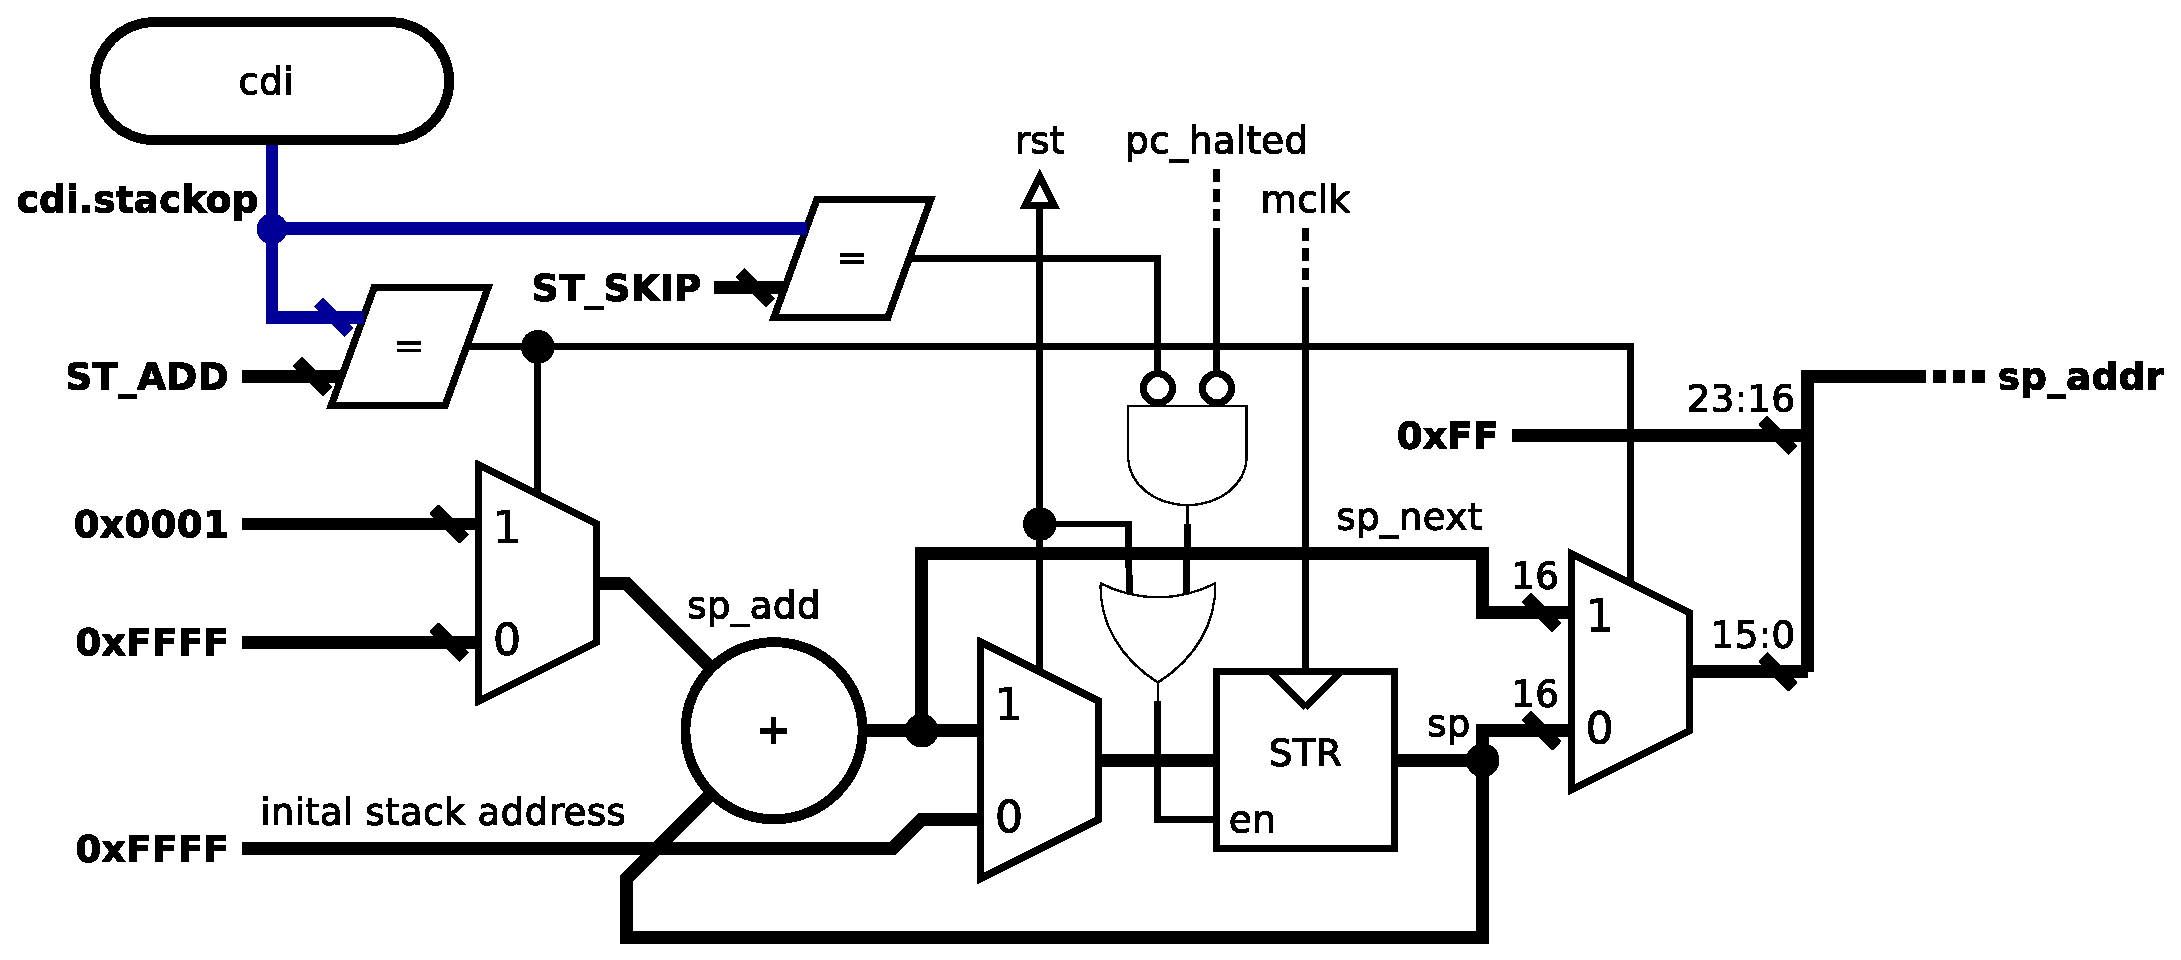
\includegraphics[scale=0.4]{graphics/stack_diagram.eps}
\caption{Digital diagram of RISC8 program counter}
\label{fig:stack_pointer}
\end{figure*}

\pagebreak
	
\begin{figure*}[ht!]
	\centering
	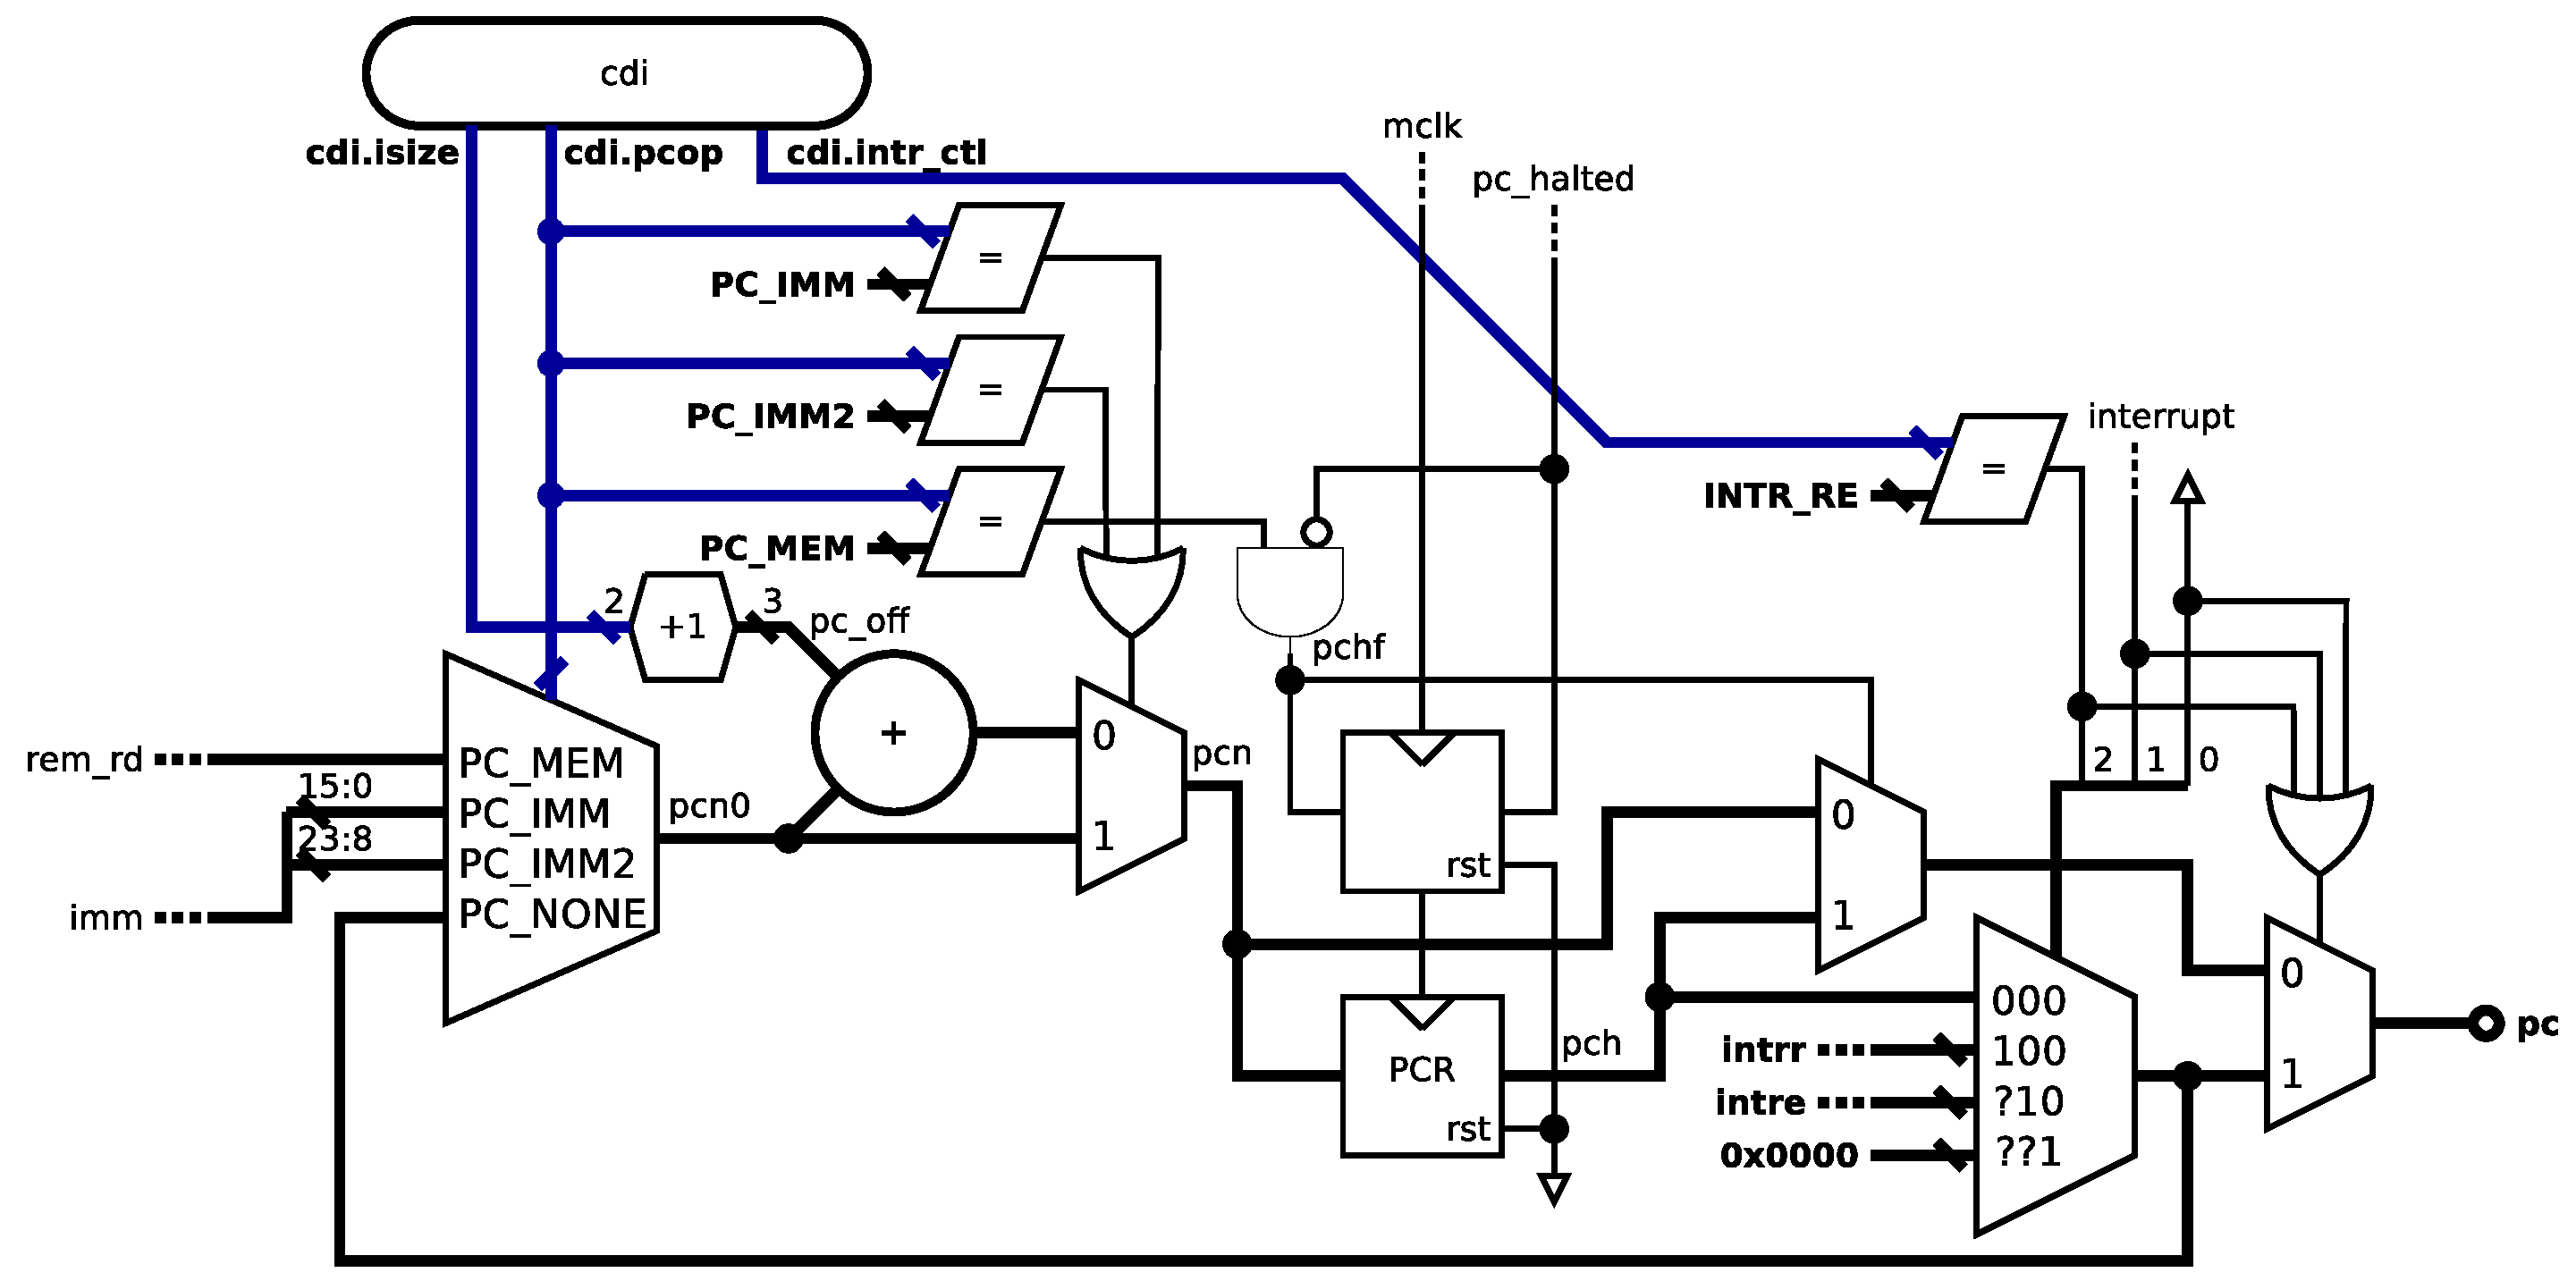
\includegraphics[width=\columnwidth]{graphics/program_counter.eps}
	\caption{Digital diagram of RISC8 program counter}
	\label{fig:program_counter}
\end{figure*}

\begin{multicols}{2}
	
\subsubsection{Stack Pointer} \label{sec:sp}
RISC processor implements stack pointer that is used in \texttt{PUSH}, \texttt{POP}, \texttt{CALL} and \texttt{RET} instructions. Stack initial address starts at highest memory address (\texttt{0xFFFF}) and subtracts 1 when data is put to stack. Figure \ref{fig:stack_pointer} represents digital diagram for stack pointer. Note that stack is only 16bit in size and most significant byte is set to \texttt{0xFF}. It also supports \textit{pc\_halted} signal from program counter to prevent stack pointer been added by 1 twice during \texttt{RET} instruction. 

One of the problems with current stack pointer implementation is 8bit data stored in 16bit memory address, wasting a byte. This can improved avoided by adding high byte register, however then it causes problems when 16bit program pointer is stored with \texttt{CALL} instruction. This can still be improved with more complicated circuit, or by using memory cache. Solution to this may be implemented in future.

\end{multicols}

\begin{figure}[h!]
	\centering
	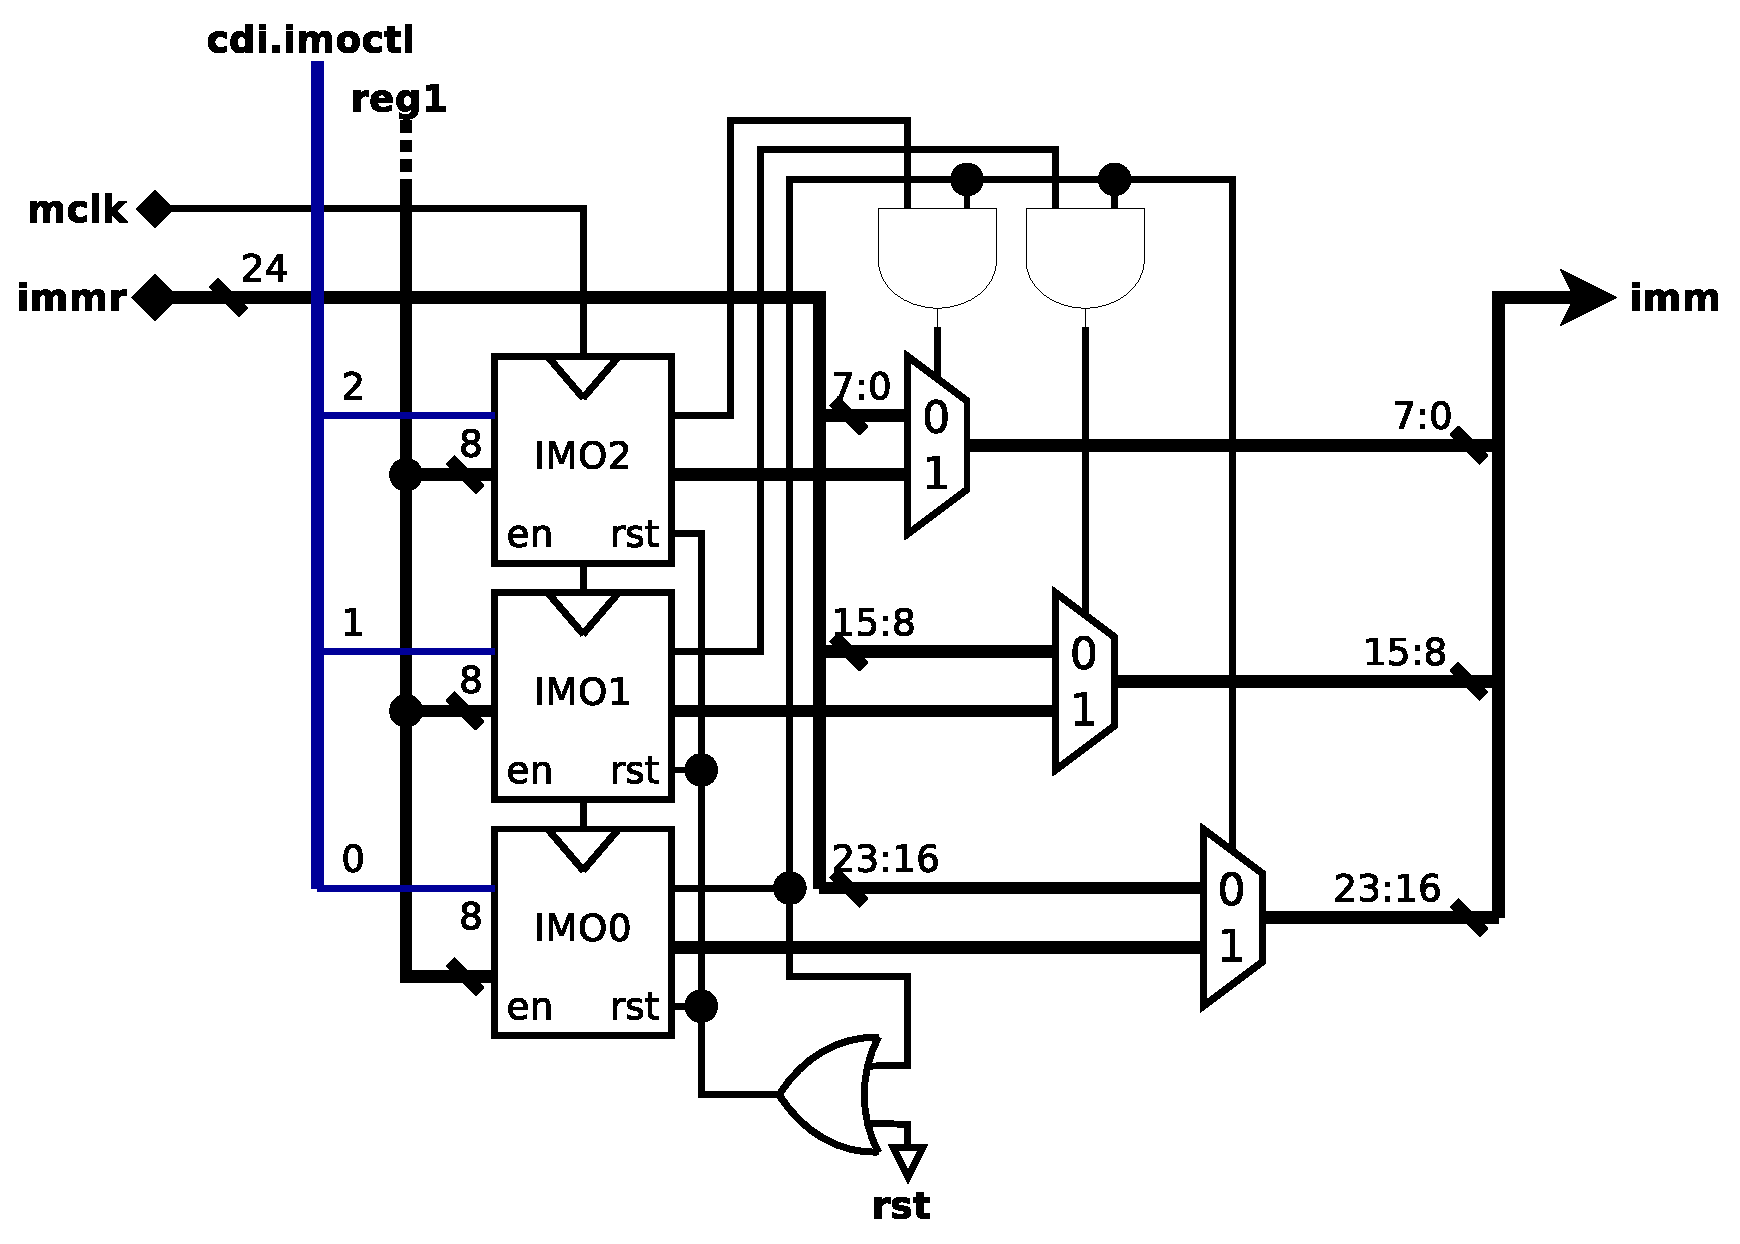
\includegraphics[scale=0.35]{graphics/imo.eps}
	\caption{Digital diagram of RISC8 immediate override logic}
	\label{fig:imo}
\end{figure}

\begin{landscape}
\subsubsection{Datapath} \label{sec:datapath}
\begin{figure}[h!]
	\centering
	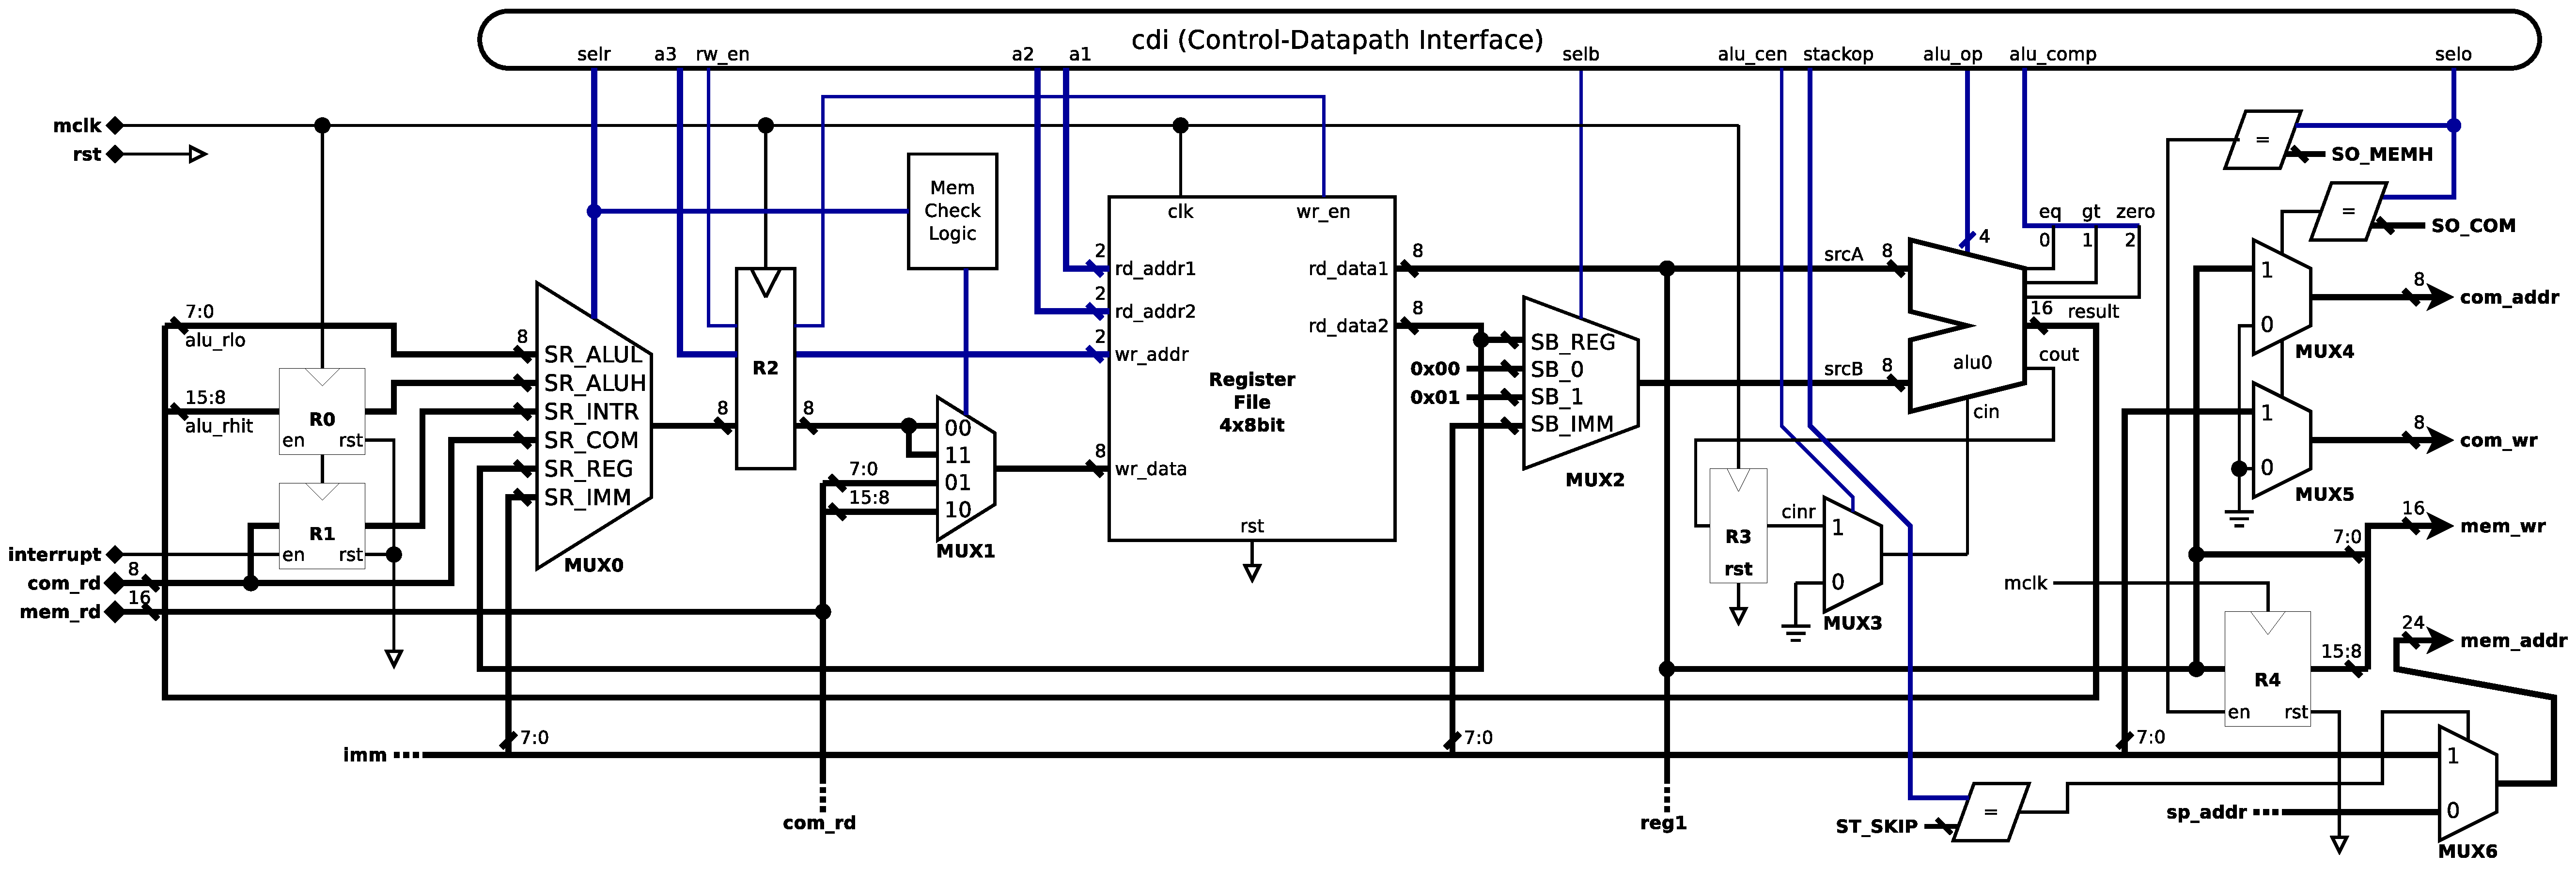
\includegraphics[width=\linewidth]{graphics/datapath.eps}
	\caption{Digital diagram of RISC8 datapath}
	\label{fig:datapath}	
\end{figure}

Figure \ref{fig:datapath} above represents partial datapath. Program counter, Stack pointer and immediate override logics are represented in figures \ref{fig:program_counter}, \ref{fig:stack_pointer} and \ref{fig:imo} respectively. CDI (Control-Data Interface) is HDL concept that connects datapath and control unit. Immediate value to datapath is provided by IMO block described in section \ref{sec:imo}.\\
Data to register file is selected and saved with \textit{MUX0}. This data is delayed 1 cycle with \textit{R2} to match timing that of data is taken from memory. If \texttt{LWLO} or \texttt{LWHI} is executed, \textit{MUX1} select high or low byte from memory to read. To compensate for timing as value written to register file is delayed by 1 cycle, register file has internal logic that outputs \textit{wr\_data} to \textit{rd\_data1} or/and  \textit{rd\_data2} immediately if \textit{wr\_en} is high and \textit{rd\_addr1} or/and \textit{rd\_addr2} matches \textit{wr\_addr}.\\
\end{landscape}
\textit{MUX2} allows override ALU source B, \textit{R3} and \textit{MUX3} enables control unit to enable ALU carry in allowing multi-byte number addition/subtraction. This function is not fully implemented yet.\textit{MUX4} and \textit{MUX5} allows to send data to COM block with \texttt{COM} instruction, if other instruction performed 0 byte for COM address and data is sent indicating no action. Data is stored in memory only with \texttt{SWLO} instruction writing to high byte whatever is stored in \textit{R4} buffer. This buffer can be written to using \texttt{SWHI} instruction. \textit{MUX6} selects memory address value from \textit{imm} or stack pointer.

\section{Summary of Difficulties and Issues}
\begin{multicols}{2}
This chapter focuses on any difficulties and issues that are hindering project from moving forward.

\subsection{List of Difficulties}

This subsection will list difficulties currently encountered:\\
\\
$\bullet$ Benchmark\\
$\bullet$ Assembler/Compiler

\subsubsection{Benchmark} \label{sec:benchmark_issues}
One of the difficulties is to design an appropriate benchmark that could test scenarios used in actual such processor applications. Other issue comes with writing benchmark itself, for instance benchmark test to finding prime number may have used many different algorithms where one of the fastest and used in actual industry may be "Sieve of Atkin" algorithm \autocite{morain_1989}, however is it fairly complicated and time consuming especially when written in assembly. 

\subsubsection{Assembler/Compiler}
In order to write more complicated code for benchmark, a proper compiler is required. Current assembler support definitions and labels, however not macros or imports from other files, nor linked libraries. Ideally, a common language compiler needs to be developed so that benchmark programs could be imported without need to completely rewrite them in assembly. However such compiler might take more time to develop than writing benchmarks in assembly. Therefore it needs to be decided which option to do.

\subsection{Failure Assessment}
This section describes likely possibilities of project failures:

As of current schedule OISC processor will be implemented in Term 2, however due to personal schedule project will be given about twice less time than in Term 1 which may result in not finishing OISC processor or developing all benchmarks for it on time. Mitigation for this is to closely follow schedule and adjust OISC design in such way as it would take less time to implement benchmark.

Another possible failure may be FPGA failure which would delay testing and benchmarking processors. This been already encountered, as JTAG caused errors while communicating with FPGA which indicated that FPGA chip is damaged. After long investigation its been discovered that problem was caused by bug in Linux JTAG Daemon service that needs to be simply restarted. Mitigation for any further issues is to have access to backup FPGA board.

\subsection{Updated Safety Risk Assessment}
There are no changes to Safety Risk Assessment.

\end{multicols}
\pagebreak

\section{Appendix A: Safety Risk Assessment}
RiskNet report is appended at the end of this document.

\section{Appendix B: Computer Code}
All code to HDL processor implementation and assembler are in git repository that can be accessed in \url{https://gogs.infcof.com/min/ucl_project_y3}

\section{References}
\printbibliography

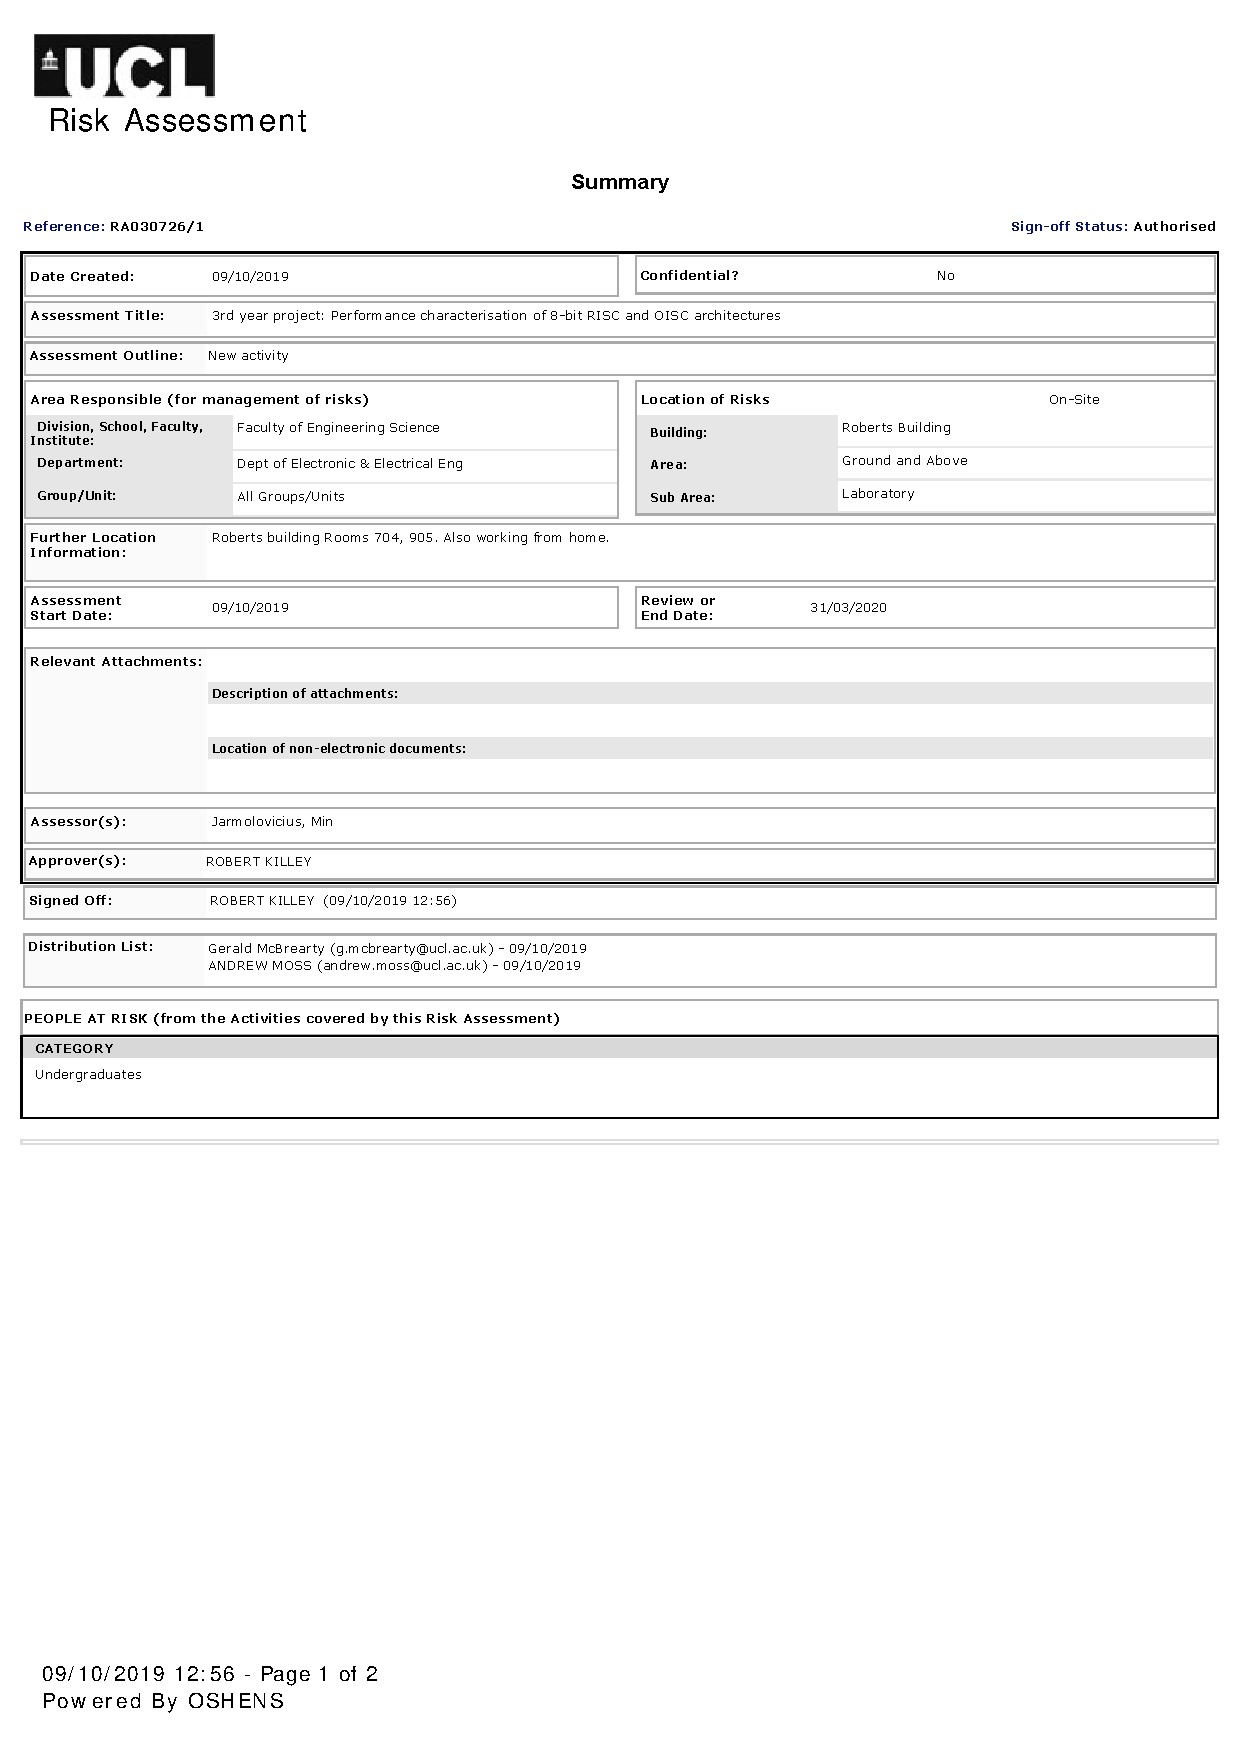
\includepdf[pages=-]{risknet.pdf}

\end{document}